\begin{figure*}[!tb]
\centering

\begin{subfigure}[b]{0.32\textwidth}
\centering
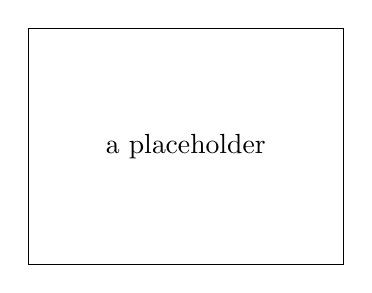
\begin{tikzpicture}
\draw (0,0) rectangle (4, 3) node [pos=0.5] {a placeholder};
\end{tikzpicture}
\caption{Subfigure 1}
\end{subfigure}
\begin{subfigure}[b]{0.32\textwidth}
\centering
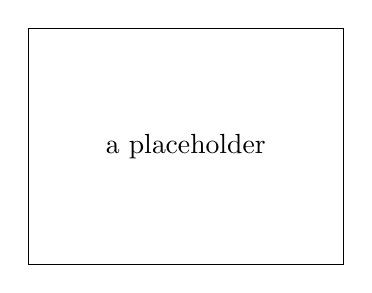
\begin{tikzpicture}
\draw (0,0) rectangle (4, 3) node [pos=0.5] {a placeholder};
\end{tikzpicture}
\caption{Subfigure 2}
\end{subfigure}
\begin{subfigure}[b]{0.32\textwidth}
\centering
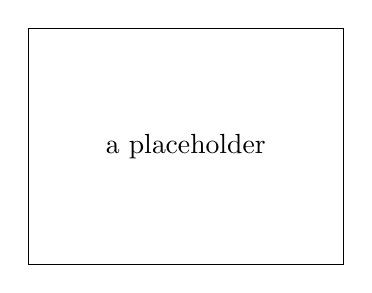
\begin{tikzpicture}
\draw (0,0) rectangle (4, 3) node [pos=0.5] {a placeholder};
\end{tikzpicture}
\caption{Subfigure 3}
\end{subfigure}
\caption{Place holders}
\end{figure*}
